\documentclass[a4paper,10pt]{article}
\usepackage[utf8]{inputenc}
\usepackage{hyperref}
\usepackage{graphicx}
\usepackage{epstopdf}

\setlength\parskip{0.25in}


\title{GPU Computing in Economics}
\author{Damian Clarke\thanks{Contact: damian.clarke@economics.ox.ac.uk}}

\begin{document}

\maketitle

\section{Introduction}
CUDA is a series of programmes and utilities designed for parallel computing 
using the Graphics Processing Unit (GPU) available in nearly all new computers.
This has been designed by NVIDIA for use with their GPUs.  NVIDIA is a brand of
GPUs used in many laptops, and is the market leader when considering dedicated 
units\footnote{Often computers will have two GPUs; one ``integrated'' unit 
which is less power intensive and is used in every day tasks, and one 
``dedicated'' unit which requires far more battery power, but which commands
its own virtual memory and has much higher performance capabilities.  It is 
these dedicated units which we focus on when undertaking parallel computing 
with the GPU.} which are suitable for parallel computation in economics (and
many other computationally intensive fields).

In a nutshell, parallel computing allows for computationally intensive 
procedures to be separated and run in individual blocks rather than as one 
large job.  This is particularly useful in applications such as Monte Carlo
simulation, or other situations in which run many processes which are mutually
independent are involved in arriving at a final result.  Historically, parallel
computation was run by splitting jobs and running them in unison over a small
number of central processing units (or CPUs) which were available to a 
computer.  However, with the advent of high powered GPUs for video games and
other graphically-demanding jobs, many more cores were made available for 
running computations.  For example, the most recent NVIDIA cards contain
upwards of 1500 cores, each of which is capable of running an individual 
computation simultaneously.

%\begin{tabular}{lcc} \hline
%\textbf{threadIdx} & unique thread ID & \\ \hline
%\end{tabular}

Host: the CPU and its memory \\
Device: the GPU and its memory\\

Location of nvcc (compiler): /usr/local/cuda-5.5/bin/nvcc
\appendix
\section{Installation}
In this appendix I describe the process that I have followed in installing and
running CUDA programs on an Optimus laptop running Ubuntu 12.04.  The laptop I 
am installing this on has an NVIDIA GeForce GT 650M Graphics card with 2GB 
gDDR3 Graphic memory.  The machine also has an integrated Intel Graphics card,
hence the need for Optimus technology to run the dedicated NVIDIA card.

Optimus technology is designed to switch seamlessly between the dedicated GPU
and integrated GPU when these both exist in the same machine.  The idea of this
is to both save power (when the dedicated GPU is not required), while taking
advantage of the dedicated GPU when higher performance is necessary.  However,
this has created some difficulties in linux based operating systems given that
many of the necessary drivers written by NVIDIA were not open source.  This
problem has been partially resolved by the 
\href{http://bumblebee-project.org/}{Bumblebee Project} which supports Optimus
under Linux.  In order to run CUDA, I ran a fresh install of Bumblebee's 
``Tumbleweed'' release (version 3.2.1).  In preparing to install CUDA, I first 
installed the most recent x-swat drivers, which bundle NVIDIA drivers for Xorg.
This follows the advice provided on the following 
\href{http://www.ivegotavirus.com/installing-bumblebee-3-0-tumbleweed-on-ubuntu/}{forum}.
and on Ubuntu looks like this:

\texttt{sudo add-apt-repository ppa:ubuntu-x-swat/x-updates} \\
\indent\texttt{sudo apt-get update} \\
\indent\texttt{sudo apt-get upgrade} \\

After installing the x-swat drivers, the current version of Bumblebee is 
installed:

\texttt{sudo add-apt-repository ppa:bumblebee/stable} \\
\indent\texttt{sudo apt-get update} \\
\indent\texttt{sudo apt-get install bumblebee} \\

At this point it is worth confirming that your Ubuntu system actually 
recognises the NVIDIA card with Optimus.  Using \texttt{lspci} allows us to see
all PCI devices in the system, and we are interested in the VGA video 
controller.  On my system I confirmed that the NVIDIA card was recognised via:

\texttt{damiancclarke@dcc-linux:~\$ lspci | grep VGA} \\
\indent\texttt{00:02.0 VGA compatible controller: Intel Corporation 3rd Gen Core processor Graphics Controller (rev 09)} \\
\indent\texttt{01:00.0 VGA compatible controller: NVIDIA Corporation GF108M [GeForce GT 630M] (rev ff)} \\

It may also be worthwhile ensuring that Bumblebee is installed correctly, by 
referring to the installation instructions and tests described
\href{https://wiki.ubuntu.com/Bumblebee#Installation}{here}.  Now, assuming 
that Bumblebee is installed correctly, we can continue by downloading the 
\href{https://developer.nvidia.com/cuda-downloads?sid=412586}{CUDA Toolkit}.
The current version (at the time of this document) is 5.5, which offers a
considerably smoother installation process than previous versions.  I largely
followed the instructions provided by NVIDIA in their
\href{http://docs.nvidia.com/cuda/cuda-getting-started-guide-for-linux/}{
Developer Zone}, however given that this is mainly intended for non-Optimus
machines, I outline the steps I followed precisely below\footnote{A more
comprehensive description is available in the aforementioned Developer Zone.
Essentially I skipped certain steps, and slightly tweaked things by using 
Optirun, but the NVIDIA documentation is much more comprehensive to what I
describe here.}: \\
\texttt{
\$ echo "foreign-architecture armhf" >> /etc/dpkg/dpkg.cfg.d/multiarch \\
\$ sudo apt-get update \\
\$ sudo dpkg -i cuda-repo-ubuntu1204\_5.5-0\_amd64.deb \\
\$ sudo apt-get update \\
\$ sudo apt-get install cuda \\
\$ export PATH=/usr/local/cuda-5.5/bin:\$PATH \\
\$ export LD\_LIBRARY\_PATH=/usr/local/cuda-5.5/lib64:\$LD\_LIBRARY\_PATH \\
}

In order to test that the above installation worked as desired, NVIDIA has 
provided a large number of sample programs.  In order to compile and run these,
I first changed to the CUDA installation directory (which in my case was
"~/usr/local/cuda-5.5/samples/") and then ran the following commands: \\
\texttt{
\$ cuda-install-samples-5.5.sh  ~
\$ cd ~/NVIDIA\_CUDA-5.5\_Samples/
\$ make
\$ cd bin/x86\_64/linux/release
\$ optirun ./deviceQuery
}

It is this final line which offers the test regarding CUDA's functionality.  If
it has installed correctly, something like the following should be seen:
\begin{figure}[htpb!]
\begin{center}
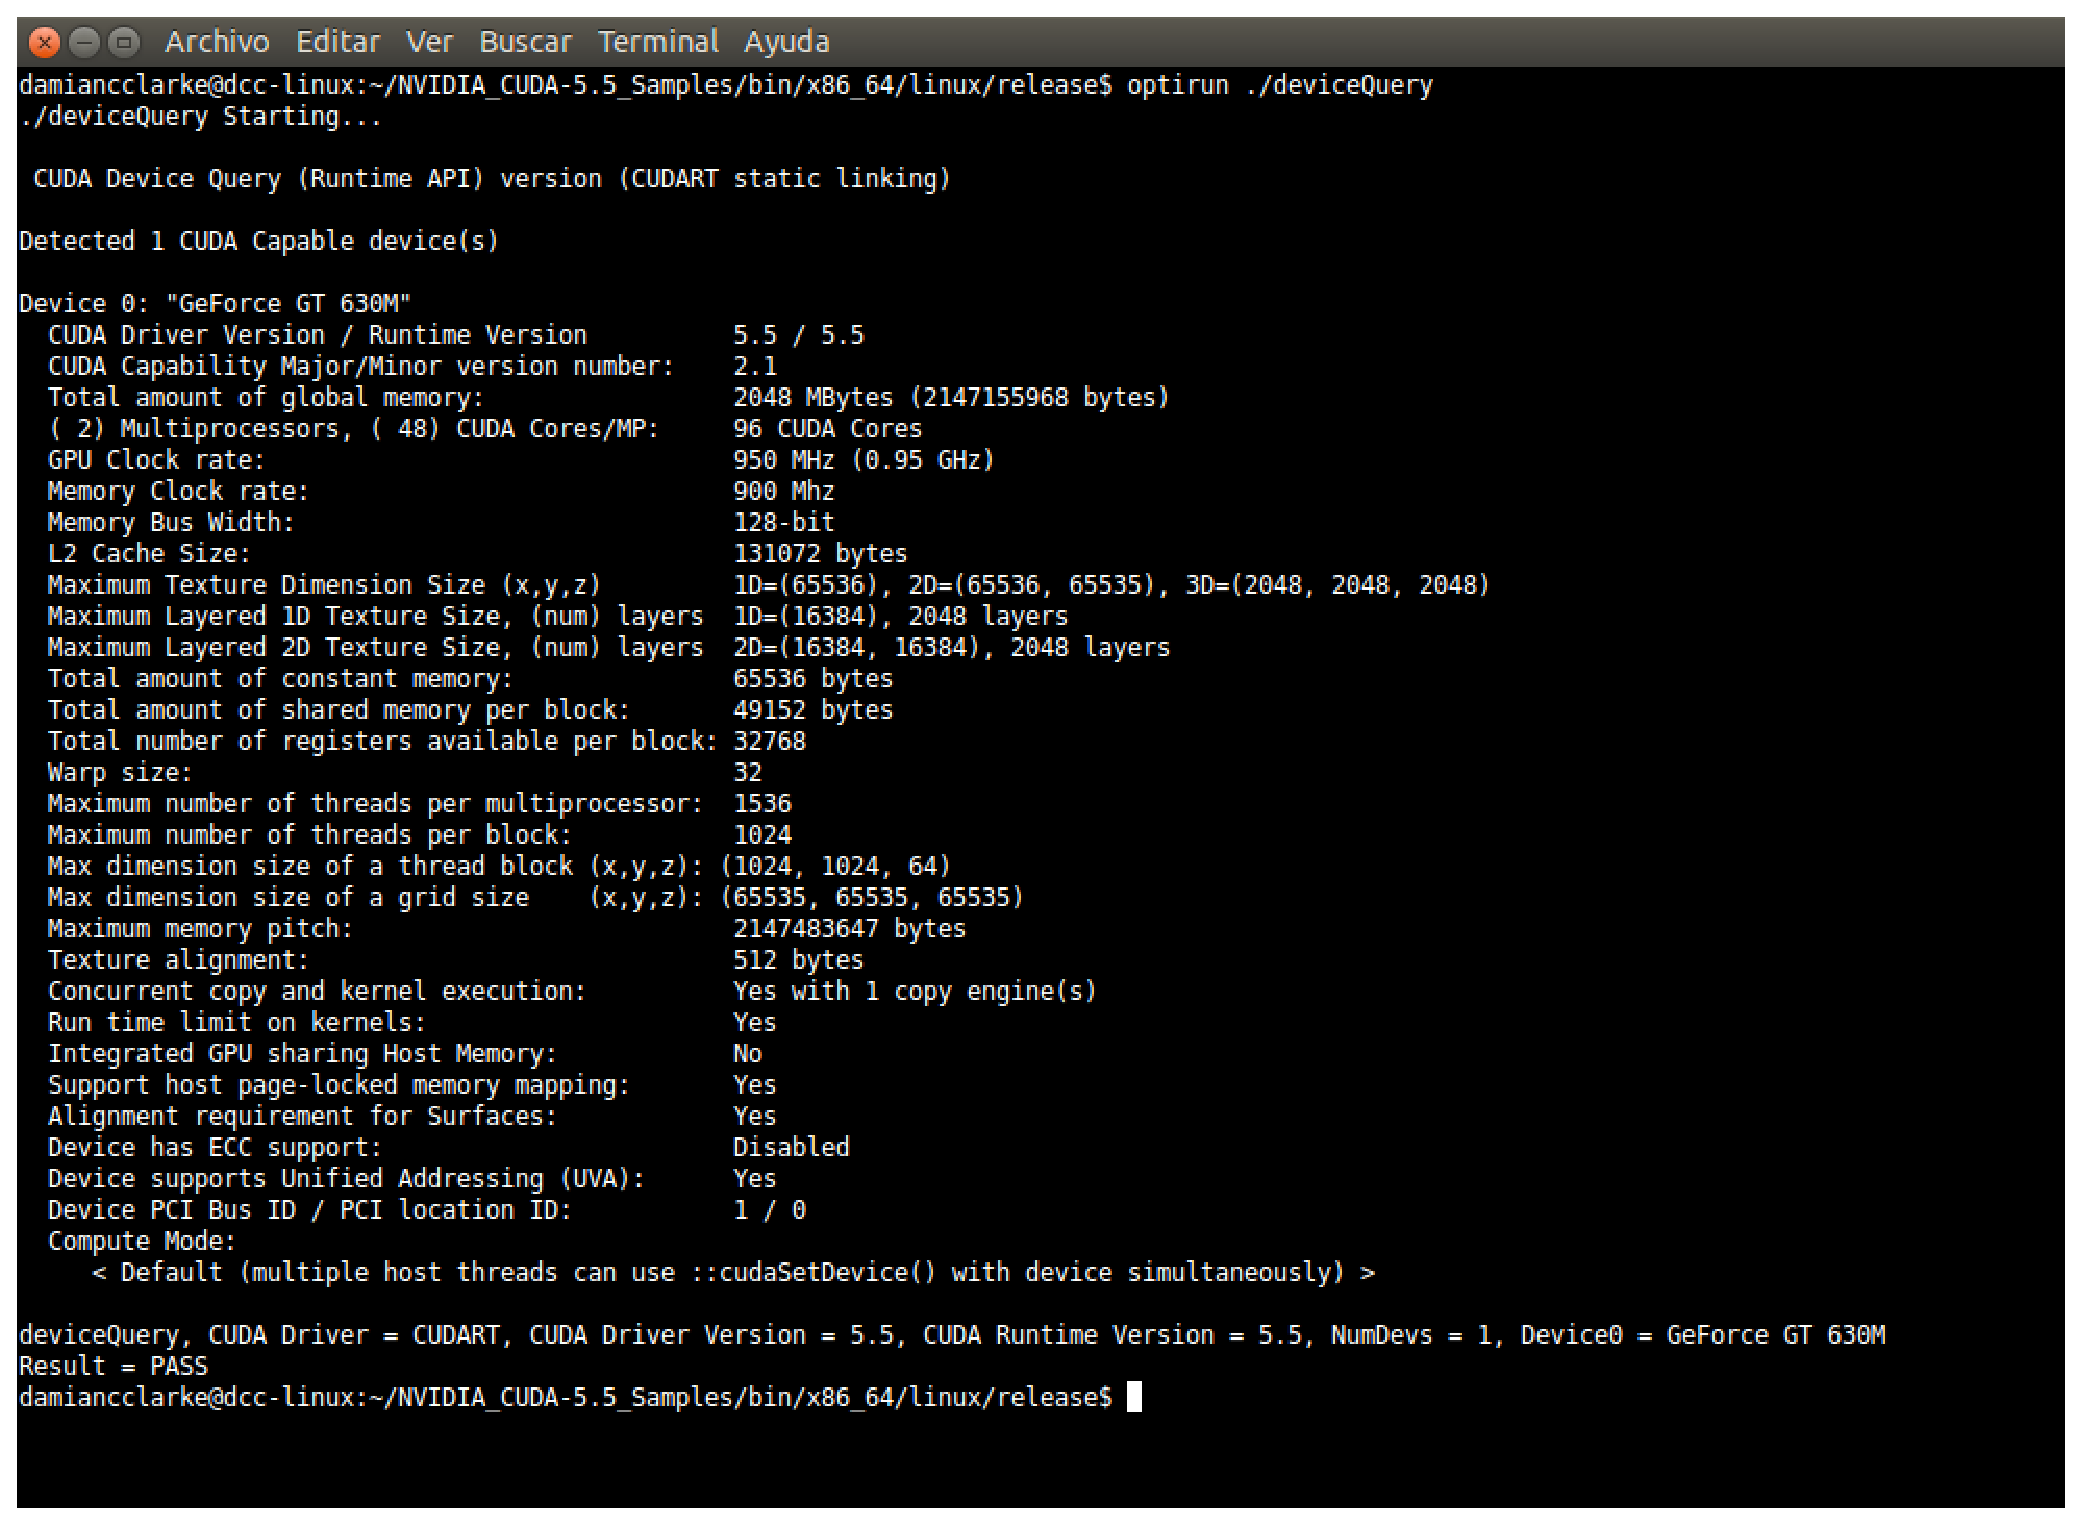
\includegraphics[scale=0.4]{devicequery.eps} 
\end{center}
\end{figure}




\end{document}
